\chapter{Build Aplikasi dan Run Pada Docker}

\section{Pembuka}
Panduan kali ini membahas cara build aplikasi dan menjalankannya pada docker. Build yang dilakukan merupakan pembuatan docker images dari Dockerfile.
Dockerfile merupakan file docker yang isinya konfigurasi yang diperlukan untuk menjalankan aplikasi. Setelah images dibuat dilakukan running aplikasi 
dengan menggunakan container. 

\begin{figure}
\section{Langkah Build Aplikasi}
1. Buat folder baru, masuk direktori folder tersebut, dan buat file bernama Dockerfile

Buat folder baru bernama dockertest:  \textcolor{Gray}{mkdir <NAMA FOLDER>}

COMMAND: \textcolor{Blue}{mkdir dockertest}

Masuk direktori folder dockertest : \textcolor{Gray}{cd <NAMA FOLDER>}

COMMAND: \textcolor{Blue}{cd dockertest}

Buat file bernama Dockerfile: 

COMMAND: \textcolor{Blue}{cat > dockertest}, Klik ENTER, klik CTRL+D
    \begin{center}
        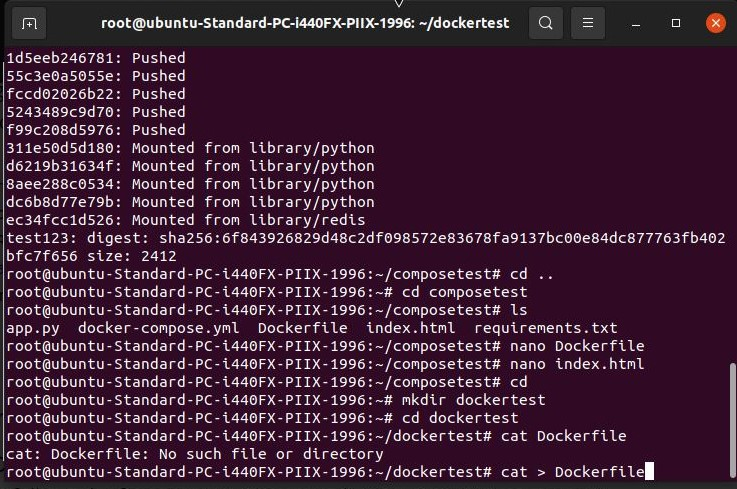
\includegraphics[width=\linewidth]{image/19.jpg}
        \caption{Buat folder dan buat dockerfile didalamnya}
        \label{fig:my_figure}
    \end{center}
\end{figure}

\begin{figure}
2. Edit file Dockerfile menggunakan editor nano dan isikan data seperti berikut 

COMMAND: \textcolor{Blue}{nano Dockerfile}
    \begin{center}
        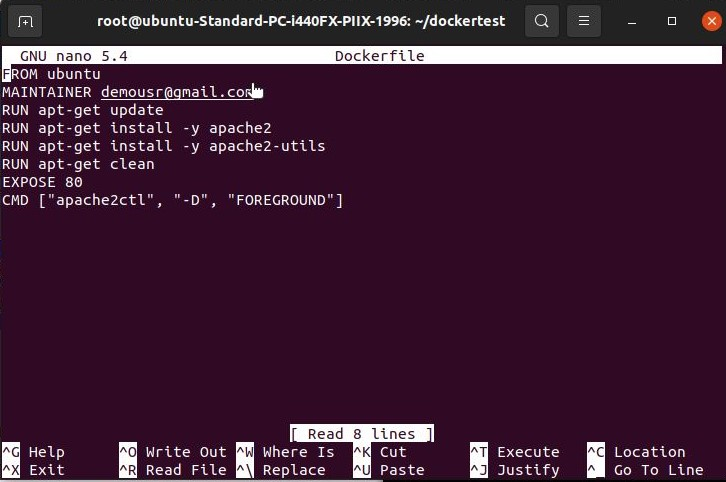
\includegraphics[width=\linewidth]{image/21.jpg}
        \caption{Isi file dockerfile}
        \label{fig:my_figure}
    \end{center}

    klik CTRL+X, klik Y, klik ENTER


    3. Build image dari Dockerfile yang sudah dibuat 

COMMAND: \textcolor{Blue}{docker build .}
    \begin{center}
        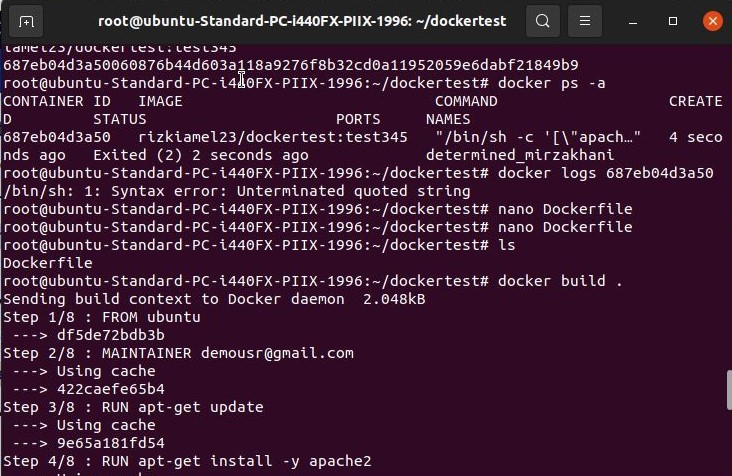
\includegraphics[width=\linewidth]{image/22.jpg}
        \caption{Build Image}
        \label{fig:my_figure}
    \end{center}
\end{figure}

\begin{figure}
4. Apabila berhasil maka akan tampil pesan Successfull built <IMAGE ID>, lalu cek daftar docker images

COMMAND: \textcolor{Blue}{docker images}
    \begin{center}
        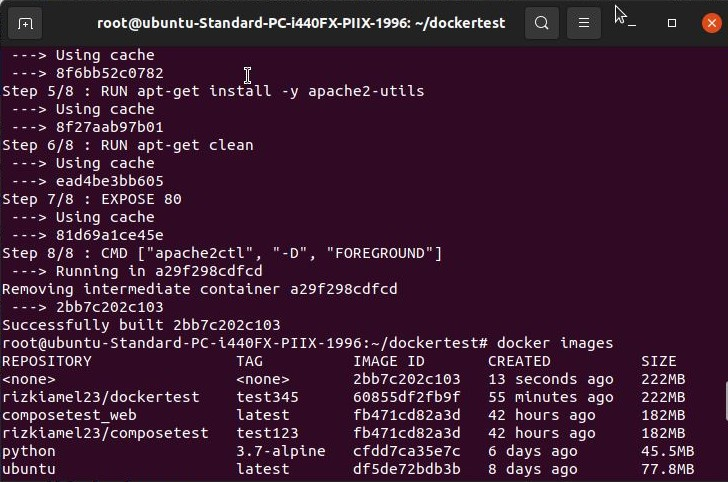
\includegraphics[width=\linewidth]{image/23.jpg}
        \caption{Cek daftar docker images}
        \label{fig:my_figure}
    \end{center}

5. Beri nama dan tag pada docker image

Beri nama dan tag : \textcolor{Gray}{docker image tag <IMAGE ID> <NAMA IMAGE:TAG>}

COMMAND: \textcolor{Blue}{docker image tag 2bb7c202c103 
rizkiamel23/dockertest2:test567}

Cek apakah nama dan tag docker images berhasil diganti :

COMMAND: \textcolor{Blue}{docker images}
    \begin{center}
        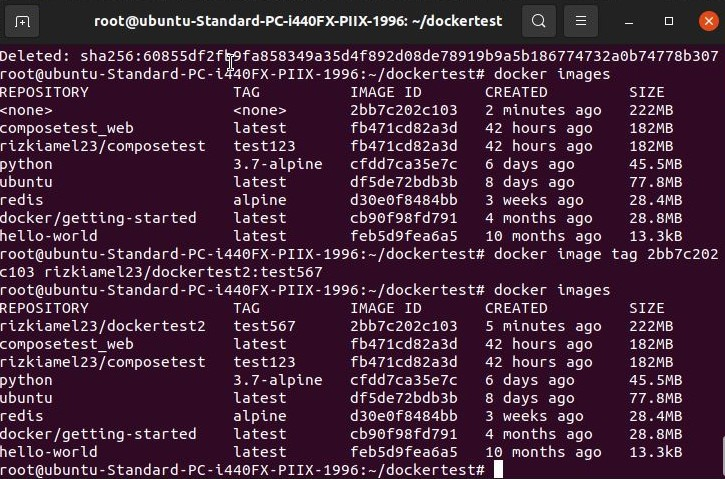
\includegraphics[width=\linewidth]{image/25.jpg}
        \caption{Tag docker images}
        \label{fig:my_figure}
    \end{center}
\end{figure}

\begin{figure}
\textcolor{BrickRed}{Keterangan : Jika ada rencana memasukan docker images pada repositori Docker / Docker Hub maka berikan nama sesuai repositori yang akan dibuat dengan format <USERNAME>/<NAMA REPOSITORI>}

\section{Run Pada Docker}

1. Buat dan run container dari docker images yang sudah dibuat

Buat dan run container dari docker images : \textcolor{Gray}{docker run <OPTION> <NAMA IMAGE:TAG>}

COMMAND: \textcolor{Blue}{docker run -dp 80:80 rizkiamel23/dockertest:test567}
    \begin{center}
        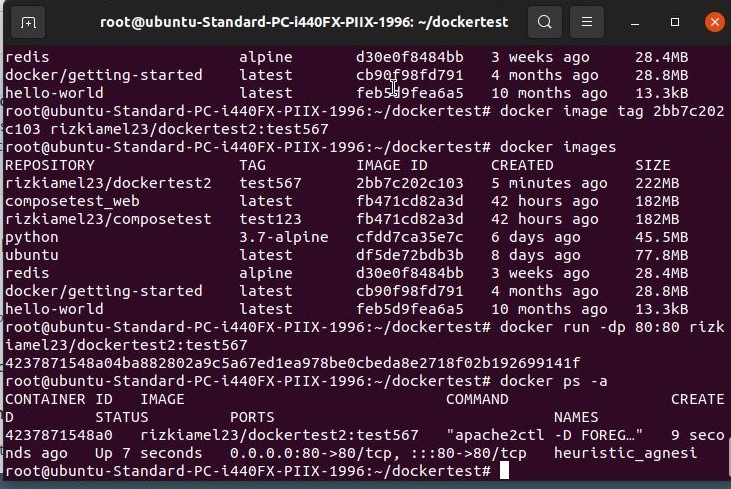
\includegraphics[width=\linewidth]{image/29.jpg}
        \caption{Buat dan run images}
        \label{fig:my_figure}
    \end{center}

\textcolor{BrickRed}{Keterangan :}

\textcolor{BrickRed}{- Opsi -d untuk mengatur ke detached mode / terpisah, agar container bisa berjalan pada background}

\textcolor{BrickRed}{- Opsi p untuk memetakan port 80 localhost yang akan mengakses port host 80 yang sudah di expose di file Dockerfile}


2. Cek apakah kontainer berjalan 

COMMAND: \textcolor{Blue}{docker ps -a}
\end{figure}
\begin{figure}
    \begin{center}
        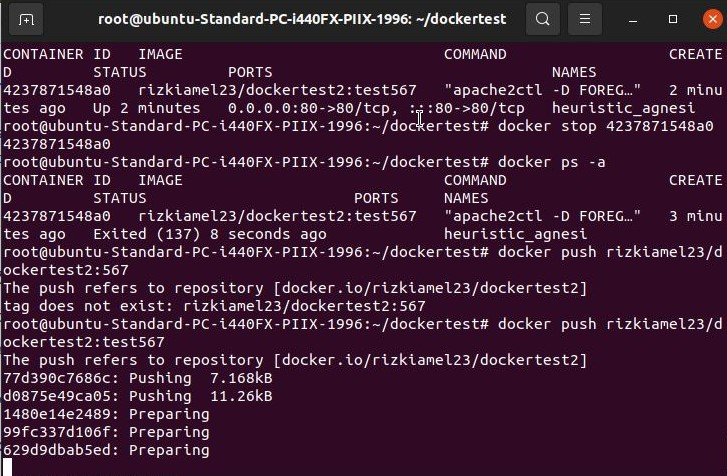
\includegraphics[width=\linewidth]{image/31.jpg}
        \caption{Cek kontainer}
        \label{fig:my_figure}
    \end{center}

Buka broser ketikan http://0.0.0.0:80
    \begin{center}
        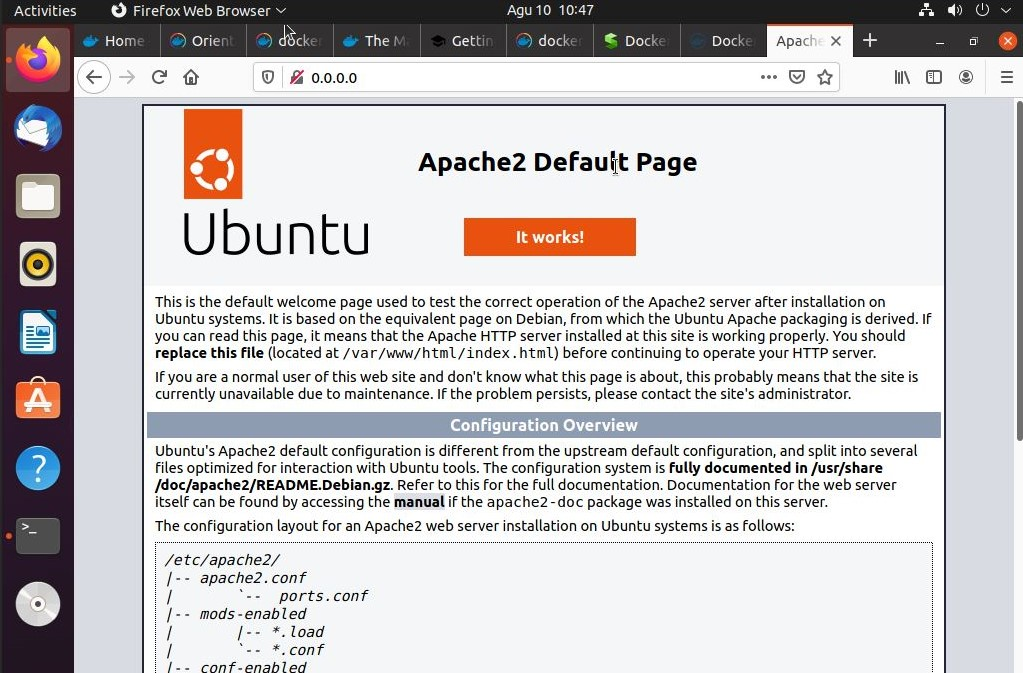
\includegraphics[width=\linewidth]{image/34.jpg}
        \caption{Tampilan akses ke kontainer}
        \label{fig:my_figure}
    \end{center}

Apabila ingin menghentikan kontainer :\textcolor{Gray}{docker stop <CONTAINER ID>}

Apabila ingin menjalankan kembali kontainer : \textcolor{Gray}{docker start <CONTAINER ID>}

Apabila ingin menghapus kontainer : \textcolor{Gray}{docker rm <CONTAINER ID>}

\end{figure}